\section{Data Product Quality Assurance} \label{sec:qa}

During PDR2, the Verification and Validation Team was responsible 
for identifying problems and bugs in the pipelines and data products. 

Here are some sample Quality Analysis Figures either selected from the 
standard V\&V Analysis plots, or generated from the PDR2 step3 (coadd) 
output images and tables.

1. \ref{fig:coadd}  

 \begin{figure}[h]
 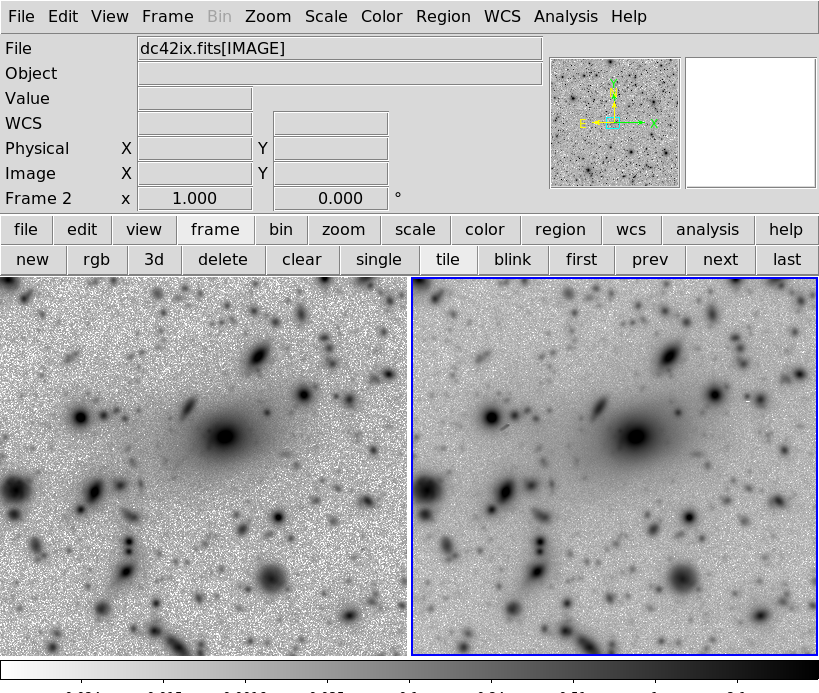
\includegraphics[width=0.9\textwidth]{sidebyside9813p42bi.png}
	 \caption{N=33 patch coadd (left) and N=300 patch coad (right).  While the visible objects are similar, the coadd to the right has less sky noise due to the deeper coadd, thus the S/N of detected objects is higher.  \label{fig:coadd}}
 \end{figure}


2. \ref{fig:s2n}

 \begin{figure}[h]
 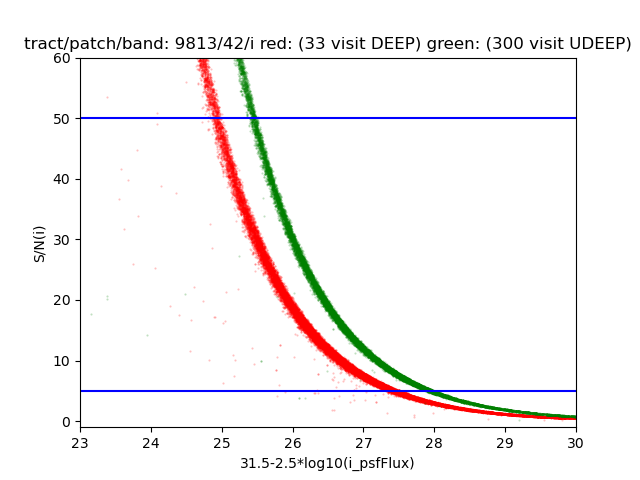
\includegraphics[width=0.8\textwidth,natwidth=600,natheight=600]{redgreen31.5.png}
	 \caption{N=33 patch coadd S/N vs. PSF mag (red) and N=300 patch coadd (green).  With the deeper coadd, the S/N for objects of the same magnitude is about 2x higher.  \label{fig:s2n}}
 \end{figure}

3. \ref{fig:colorcolor}

 \begin{figure}[h]
 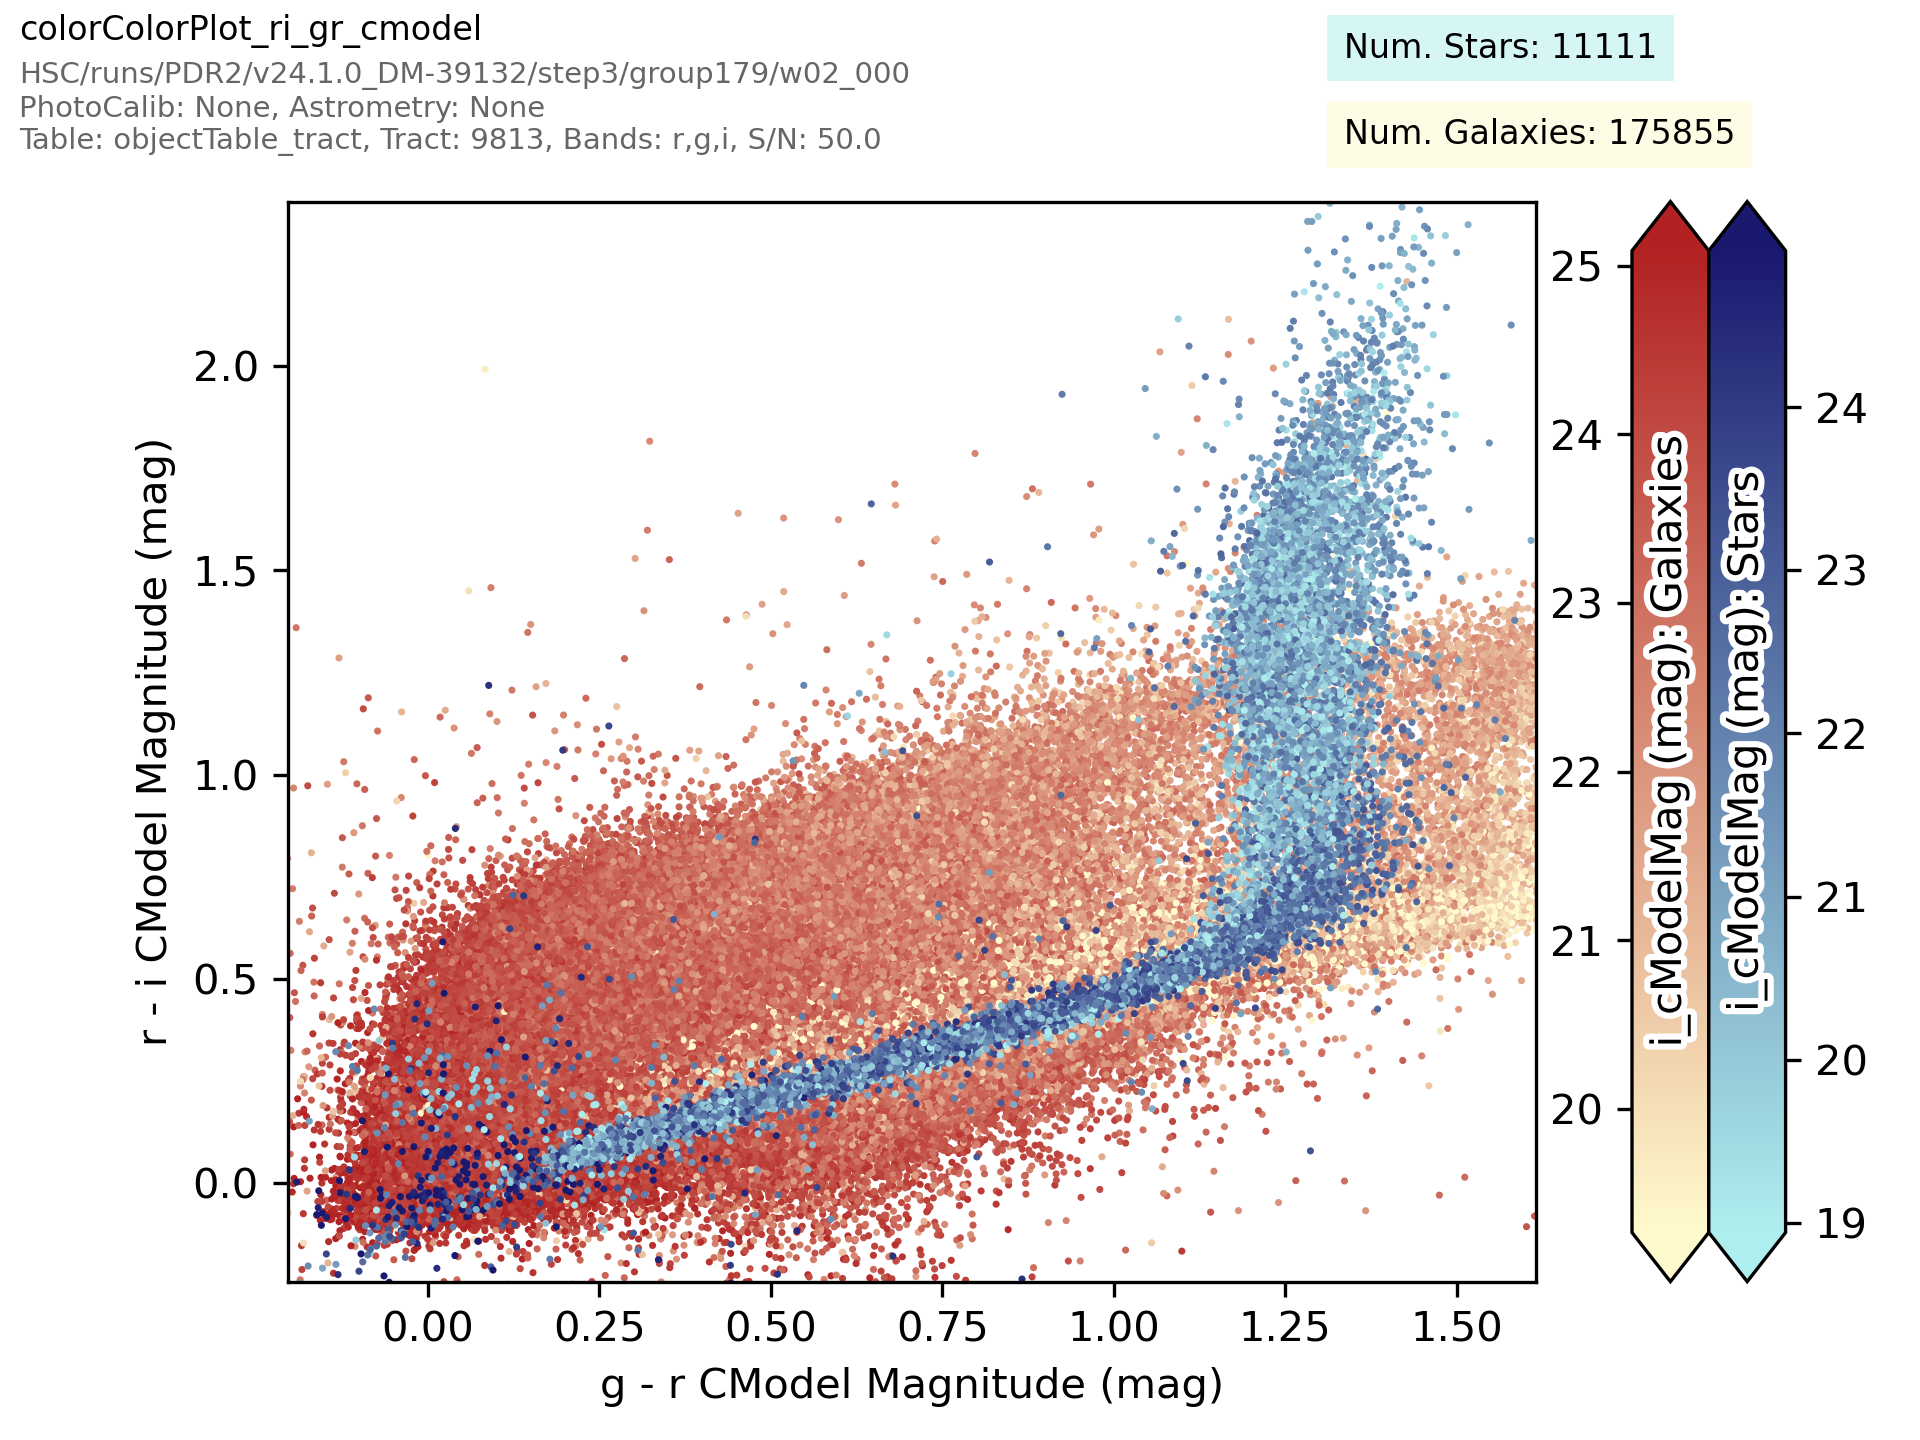
\includegraphics[width=0.9\textwidth]{colorColor9813.png}
	 \caption{Color color plot of objects masured in UDEEP COSMOS tract 9813 with star/galaxy separation (N=300).  \label{fig:colorcolor}}
 \end{figure}

4. \ref{fig:deblend1}

 \begin{figure}[h]
 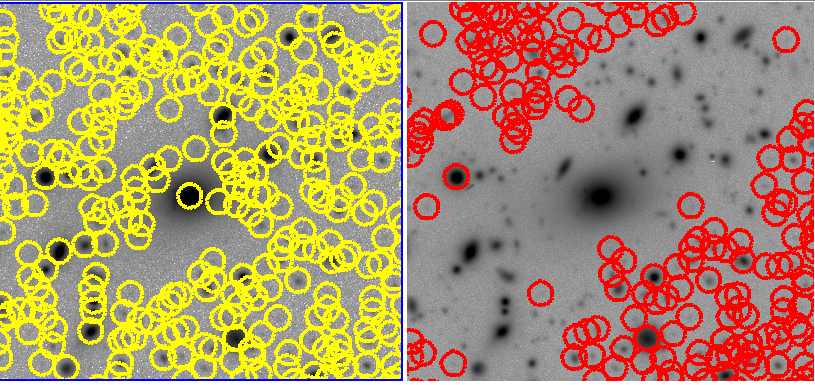
\includegraphics[width=0.9\textwidth]{wobjects.png}
	 \caption{N=33 patch coadd (left) and N=300 patch coad (right).  Here the deblending or detection of objects in the very deep coadd misses some objects in the wings of bright central galaxies or bright stars.  \label{fig:deblend1}}
 \end{figure}

5. \ref{fig:deblend2}

 \begin{figure}[h]
 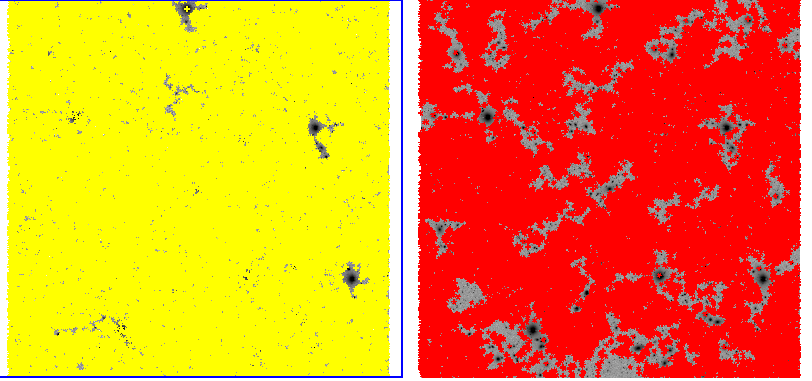
\includegraphics[width=0.9\textwidth]{full.png}
	 \caption{N=33 patch coadd (left) and N=300 patch coad (right).  Here the deblending or detection of objects in the very deep coadd misses some objects in the wings of bright central galaxies or bright stars.  \label{fig:deblend2}}
 \end{figure}

6. \ref{fig:deblend3}

 \begin{figure}[h]
 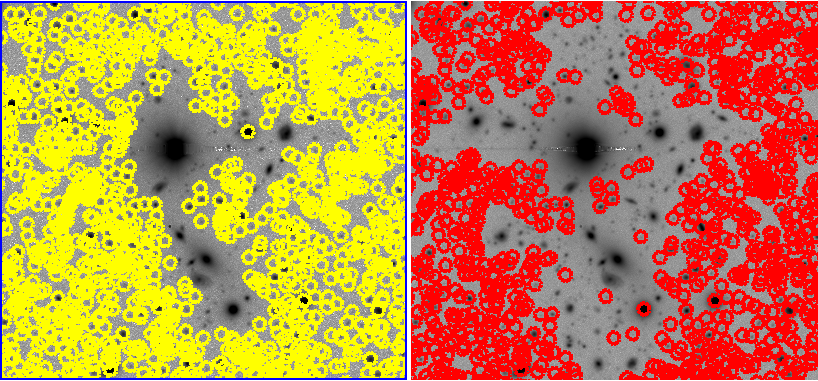
\includegraphics[width=0.9\textwidth]{deblend.png}
	 \caption{N=33 patch coadd (left) and N=300 patch coad (right).  Here the deblending or detection of objects in the very deep coadd misses some objects in the wings of bright central galaxies or bright stars.  \label{fig:deblend3}}
 \end{figure}

There were there main phases of V\&V work:

\begin{itemize}
\item A period of analysis using a “pilot run” before the start of production, which ran a single
tract through all steps of the pipeline, using the codebase planned for the release.
\item Two “gates”, one at the end of single frame processing and another after coadd construction,
where production was halted for V\&V to confirm that all the data products were ready before moving
on to the next step of processing.
\item Spot checks during processing, and follow-up of unexpected errors or failed tasks.
\end{itemize}

During these main phases, the V\&V team made extensive use of the plotting capabilities in
analysis\_drp along with adding new diagnostic plots. Much of the analysis was performed by writing
notebooks to test out new diagnostics for data products that were recently added to the pipelines.
The team also drew on experience from many prior processings (particularly of Hypersuprime-cam) to
quickly distinguish ``known'' problems from new problems.

A notable success occurred during coadd construction, when as part of the spot checks during
processing the team noticed some regions inside successfully-processed patches had no coadd sources
detected. One of the plots that lead to this discovery is shown below. This was particularly
unexpected because entire patches are expected to succeed or fail entirely, it was highly unusual
for portions to fail silently.

The eventual explanation was that the coaddition code operated on sub-patch-sized regions
sequentially, in order to limit peak memory usage, and so it would read from disk different portions
of the input warp images as it progressed. On a typical POSIX filesystem these reads typically
either all succeed or all fail, but in the cloud environment the object store would sometimes deny
individual requests as a form of rate-limiting. The coaddition code could have caught this, but
since that type of failure was never encountered in prior usage, it mistakenly proceeded without
raising an exception. Because this issue was identified early during coaddition, only a few days
worth of processing had to be redone.










\ref{fig:footprint1} shows the whole footprint of the processed PDR2
dataset

 \begin{figure}[h]
 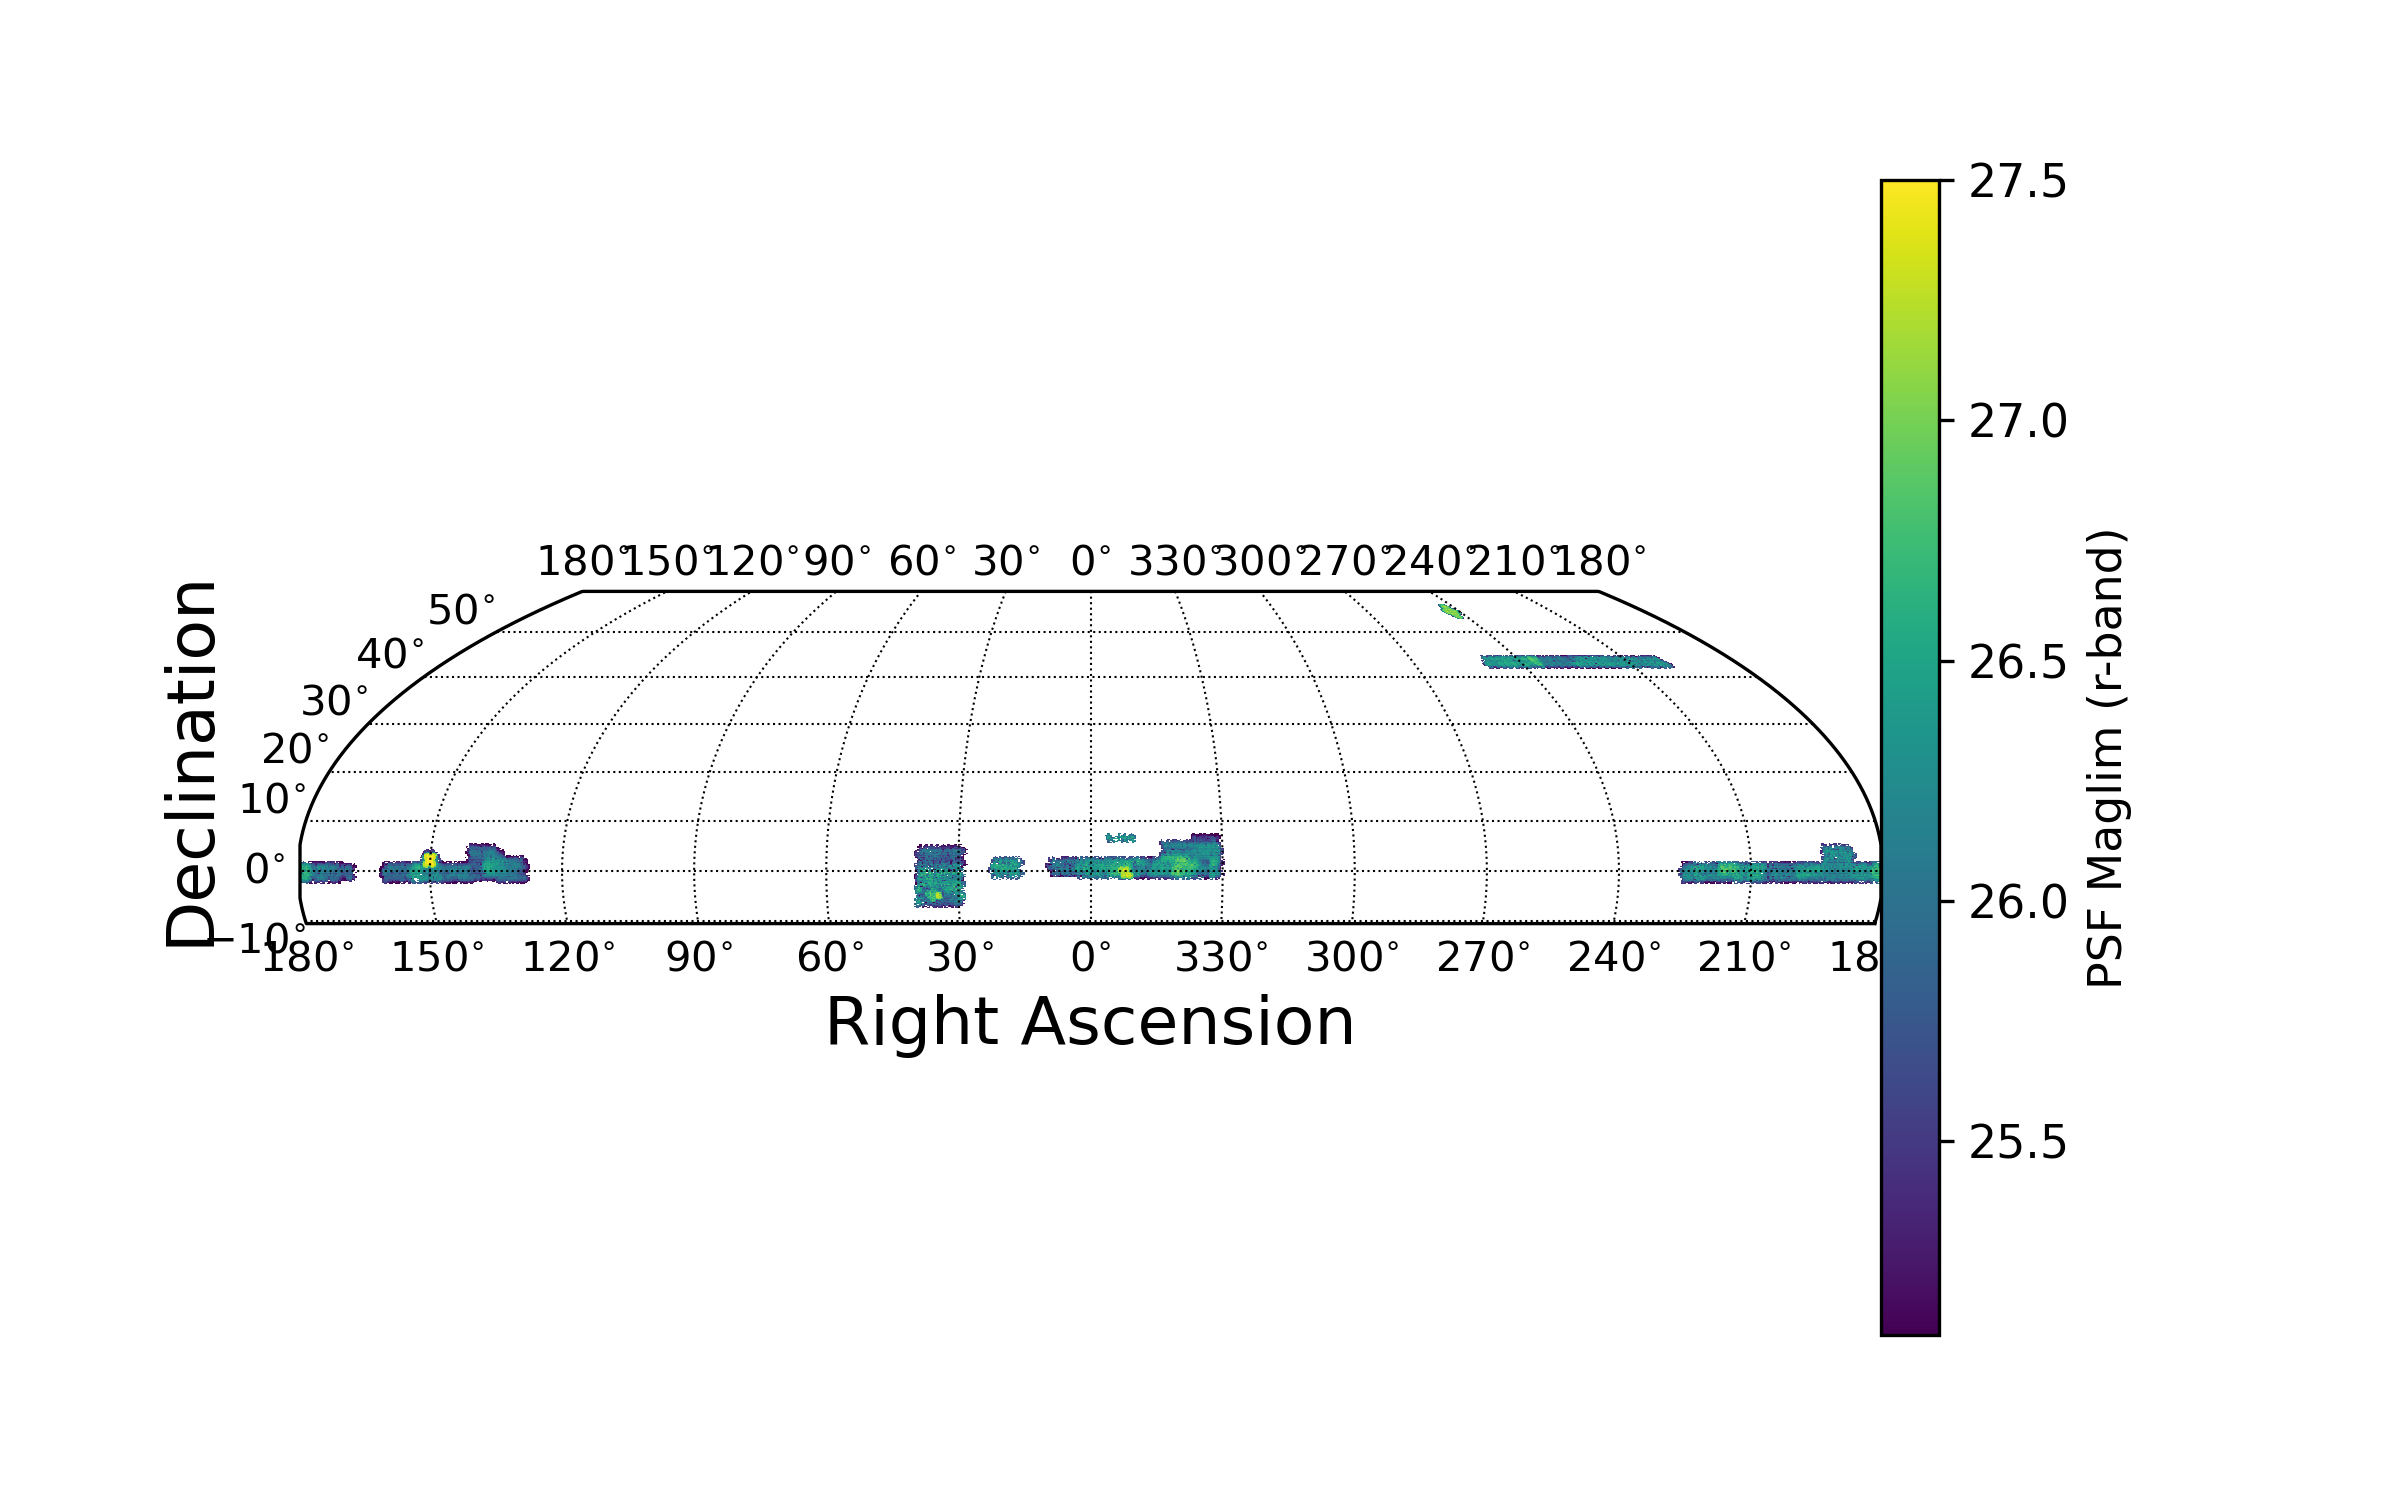
\includegraphics[width=0.9\textwidth]{r_maglim_pdr2.png}
	 \caption{Footprint of PDR2 dataset.  \label{fig:footprint1}}
 \end{figure}

 \ref{fig:footprint0} shows a close up of a figure derived from the healSparsePropertyMap for coadded sky noise of the footprint, scaled to reflect point
 source detection limit in each healpix pixel of the sky.

 \begin{figure}[h]
 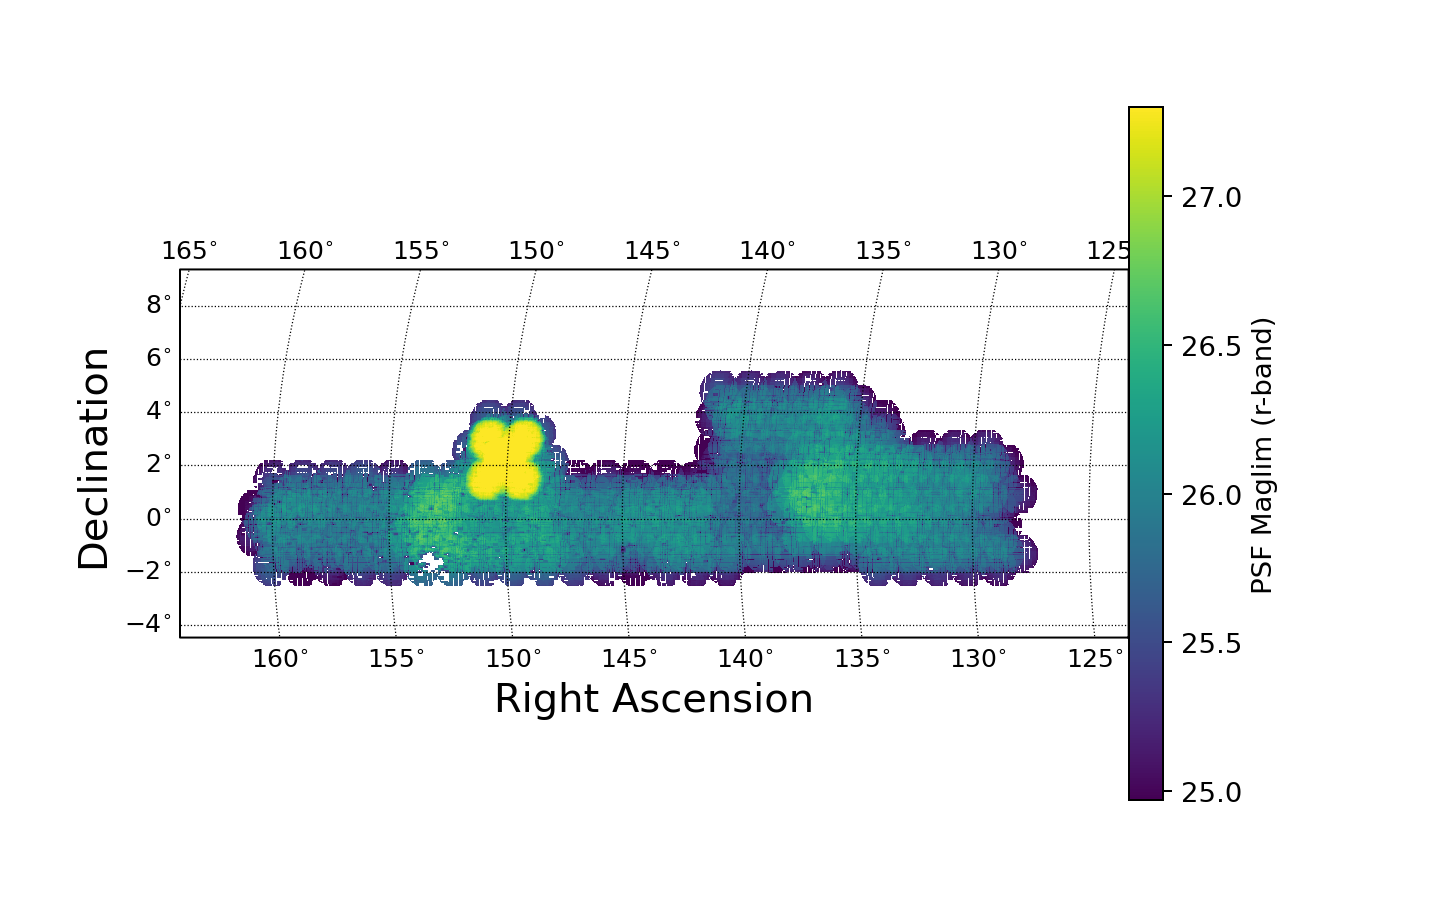
\includegraphics[width=0.9\textwidth]{r-band-cosmos-pdr2.png}
	 \caption{Closeup of PDR2 footprint depth near the COSMOS UDEEP tract.  \label{fig:footprint0}}
 \end{figure}

The data previews are also a chance to learn from the issues that we didn’t catch during V\&V; most
notably were two cases where invalid flux calibrations were being applied to certain measurement
algorithms, resulting in NaNs in the output. This case shows the value of having a wide breadth of
testing coverage. For future releases we will ensure that we have some form of testing for every
column in every user-facing data product. Even if the tests are relatively simple, they may identify
significant issues.

As one further example of potential issues encountered during production, a few days after the start
of single frame processing the pipelines began to show hundreds of failures with the error message
\texttt{Exception ValueError: No reference objects supplied}. This was not seen in the pilot run, so
production was paused while we investigated. By plotting the locations of these failures on the sky,
we determined that these sensors fell outside the footprint of the stellar input catalog, and hence
there were no stars available for calibrating these images. These were thus “unprocessable” and no
corrective action was required, but it illustrated the value of realtime error collection and
monitoring during production.

